%% LyX 2.2.3 created this file.  For more info, see http://www.lyx.org/.
%% Do not edit unless you really know what you are doing.
\documentclass[english]{article}
\usepackage[T1]{fontenc}
\usepackage[latin9]{inputenc}
\usepackage{geometry}
\geometry{verbose,tmargin=1in,bmargin=1in,lmargin=1in,rmargin=1in,headheight=0in,headsep=0in}
\usepackage{color}
\usepackage{babel}
\usepackage{graphicx}
\usepackage[unicode=true]
 {hyperref}

\makeatletter

%%%%%%%%%%%%%%%%%%%%%%%%%%%%%% LyX specific LaTeX commands.
%% Because html converters don't know tabularnewline
\providecommand{\tabularnewline}{\\}

%%%%%%%%%%%%%%%%%%%%%%%%%%%%%% Textclass specific LaTeX commands.
\newenvironment{lyxcode}
{\par\begin{list}{}{
\setlength{\rightmargin}{\leftmargin}
\setlength{\listparindent}{0pt}% needed for AMS classes
\raggedright
\setlength{\itemsep}{0pt}
\setlength{\parsep}{0pt}
\normalfont\ttfamily}%
 \item[]}
{\end{list}}

\makeatother

\begin{document}

\title{CSCE 221 Cover Page\\
 Programming Assignment \#6 \\
Due \textbf{April 29} by midnight to eCampus}

\author{First Name~Hunter~~~~~~Last Name ~~~~Cleary~~~~UIN~~~625001547~~~}

\date{User Name ~~~hncleary~~~~~E-mail address~~~hncleary@tamu.edu~~~~~\medskip{}
}
\maketitle
\begin{quotation}
Please list all sources in the table below including web pages which
you used to solve or implement the current homework. If you fail to
cite sources you can get a lower number of points or even zero. According
to the University Regulations, Section 42, scholastic dishonesty are
including: acquiring answers from any unauthorized source, working
with another person when not specifically permitted, observing the
work of other students during any exam, providing answers when not
specifically authorized to do so, informing any person of the contents
of an exam prior to the exam, and failing to credit sources used.
Disciplinary actions range from grade penalties to expulsion read
more: \href{http://aggiehonor.tamu.edu/}{Aggie Honor System Office}
\medskip{}
\medskip{}
\end{quotation}
\begin{center}
\begin{tabular}{|c|c|c|c|}
\hline 
Type of sources  & ~~~~~~~~~~~~~~~~~~~~~~~ & ~~~~~~~~~~~~~~~~~~~~~~~~ & ~~~~~~~~~~~~~~~~~~~~~~~\tabularnewline
 &  &  & \tabularnewline
\hline 
\hline 
People &  &  & \tabularnewline
 &  &  & \tabularnewline
\hline 
Web pages (provide URL)  & URLS Listed Below &  & \tabularnewline
 &  &  & \tabularnewline
\hline 
Printed material & Data Structures and Algorithms  & Programming P\&P C++ & \tabularnewline
 & (Textbook) & (Stroustrup)  & \tabularnewline
\hline 
Other Sources  &  &  & \tabularnewline
 &  &  & \tabularnewline
\hline 
\end{tabular}
\par\end{center}
https://en.wikipedia.org/wiki/Associative\_array\ \\
https://www.hackerearth.com/practice/data-structures/hash-tables/basics-of-hash-tables/tutorial/\ \\
http://www.cplusplus.com/reference/sstream/stringstream/stringstream/\ \\
http://www.cplusplus.com/reference/vector/vector/erase/\ \\
http://www.cplusplus.com/reference/map/map/operator[]/\ \\
http://www.cplusplus.com/reference/map/map/count/\ \\
\ \\
\medskip{}
\medskip{}
\begin{quotation}
I certify that I have listed all the sources that I used to develop
the solutions/codes to the submitted work.

\textquotedblleft On my honor as an Aggie, I have neither given nor
received any unauthorized help on this academic work.\textquotedblright{} 
\end{quotation}
\bigskip{}
\bigskip{}

\begin{tabular}{cccccc}
Your Name  & ~~~Hunter~~Cleary~~~ &  & ~~~~~~~~~~~~~~~~~~~~~ & Date  & ~~~~4/29/18~~~~~\tabularnewline
\end{tabular}\newpage{}
\noindent \begin{center}
\textbf{\Large{}Programming Assignment \#6}
\par\end{center}{\Large \par}

\noindent \begin{center}
{\large{}Due }\textbf{\emph{\large{}April 29}}{\large{} to submit
to eCampus\medskip{}
}
\par\end{center}{\large \par}
\item \textbf{Report}
\begin{enumerate}
\item Explain how your brackets operator works.
\begin{enumerate}
\item What is the running time expressed in terms of big-Oh asymptotic notation
of your brackets operator?\ \\
\ \\
The brackets operator runs in $O(logn)$ time.
\ \\
\item How could you improve the running time? Here don\textquoteright t
think about micro optimizations, think about changing data structures
or major algorithm changes. \ \\
\ \\
To improve the running time, implement a different data structure. If keys were replaced with integer values, the elements could be accessed in vector in constant time $O(1)$. 

\ \\
\end{enumerate}
\item Explain what the advantages and disadvantages of implementing map
with the following data structures 
\begin{enumerate}
\item A vector of key\_values b. \ \\
\ \\
A vector of key\_values allows for a conceptually easy design. Iterating through data is simple. Buidling the vector of keys can be done in linear time. Very useful if keys are already sorted.
\ \\
\item A tree of key\_values. 
\begin{enumerate}
\item Regular binary\ \\
\ \\
Allows for key search in logarithmic time. Although building the tree will take more time, computing time is conserved when looking up keys. 
\ \\
\item Red Black\ \\
\ \\
Similar to the regular binary tree but is self-balancing. The managed height of the tree would result in faster key search times. This data structure is good to use if keys need to be deleted and added frequently.
\ \\
\item AVL \ \\
\ \\
Another self-balancing binary tree. Managed height would result in faster key search times. Most useful when the task being completed requires extensive numbers of key searches.
\ \\
\item 2-4 \ \\
\ \\
Another self-balancing tree. Allows for multiple child nodes. Like red-black trees, it is most useful when a larger number of keys need to be deleted or added.
\ \\
\end{enumerate}
\item A Hash Table of key\_values\ \\
\ \\
Hash tables are useful when implementation of a hash function is needed. Would be most useful when the keys being inserted are not skewed, resulting in a lower number of collisions. Accessing keys would have a constant time average, but a linear worst case. Hash tables are efficient in storing bound keys in a structure, but lack the sorting of the other structures.
\ \\
\end{enumerate}
\item Explain one real life use case for a map, you should say specifically
why it would benefit from using a map over a simpler data structure
like a vector. This doesn\textquoteright t have to be something that
exists currently, it\textquoteright s just an idea for how you could
use a map. Example (don\textquoteright t use this one) storing word
frequencies for a large document. \ \\
\ \\
A real life usage for a map data structure would be an interest profile for users on a website. The map could keep track of the frequency of related data that has been viewed in clusters. Using the frequencies, a profile could be created so that the content and advertisements shown to the user are catered to their interests.\ \\
\ \\
\textbf{Charts and Tables}\ \\
\ \\
\textbf{Unfiltered}\ \\
\ \\
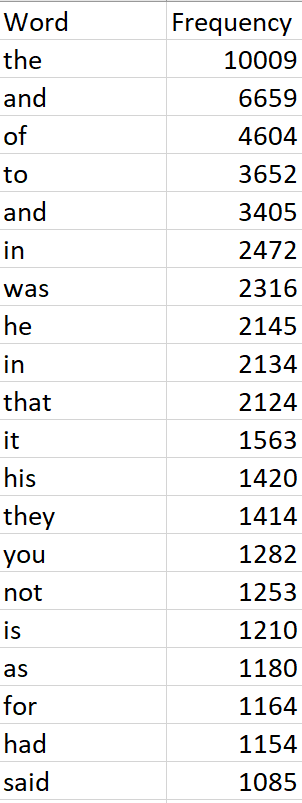
\includegraphics[height = 8cm]{FrequencyOfWordsUnfiltered-Table.png}
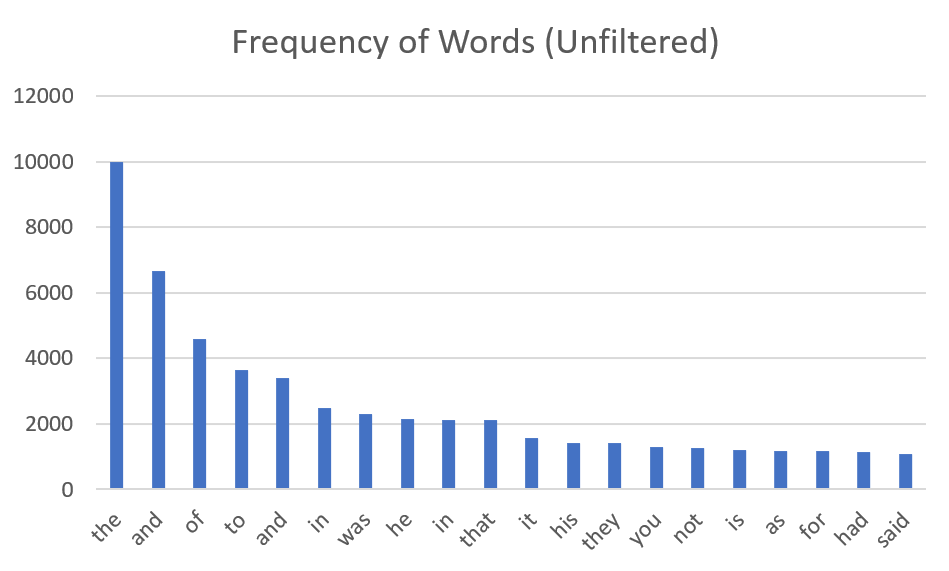
\includegraphics[width = 12cm]{FrequencyOfWordsUnfiltered.png}
\ \\
\textbf{Filtered}\ \\
\ \\
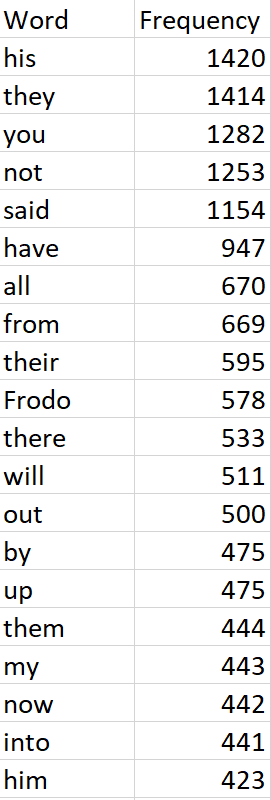
\includegraphics[height = 8cm]{FrequencyOfWordFiltered-Table.png}
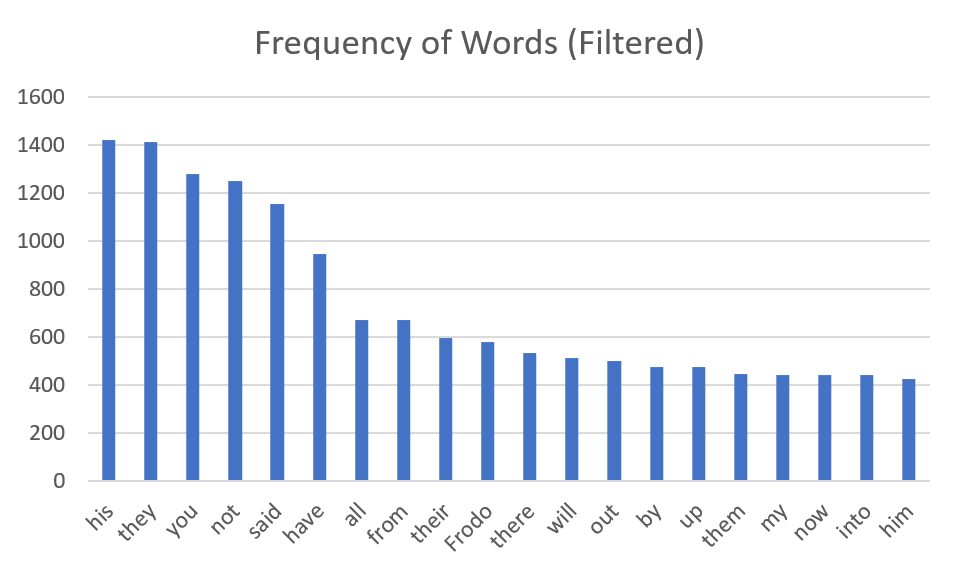
\includegraphics[width = 12cm]{FrequencyOfWordFiltered.png}
\ \\
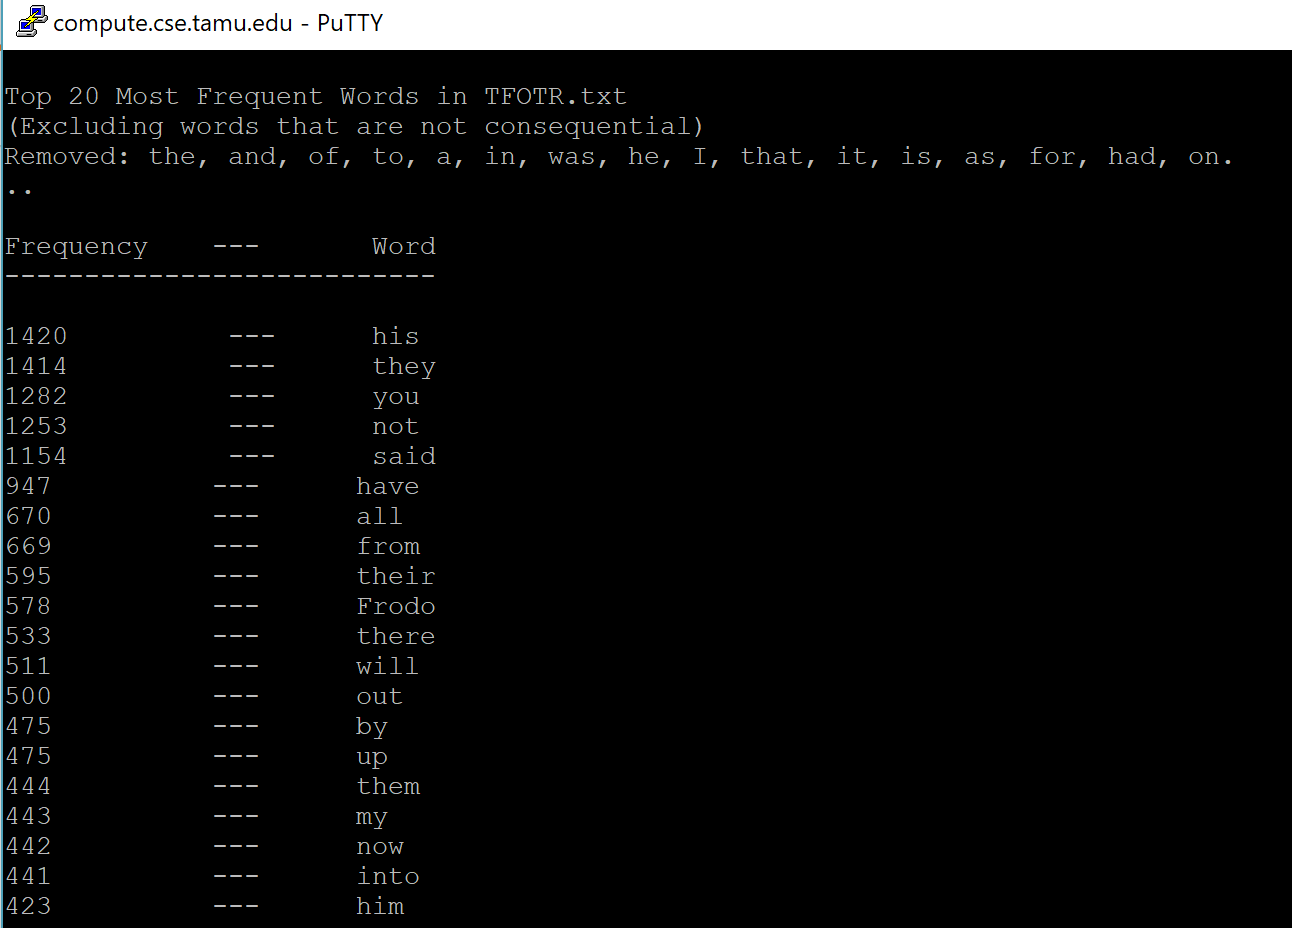
\includegraphics[width = 8 cm]{PUTTYBuildServerOutput.png}
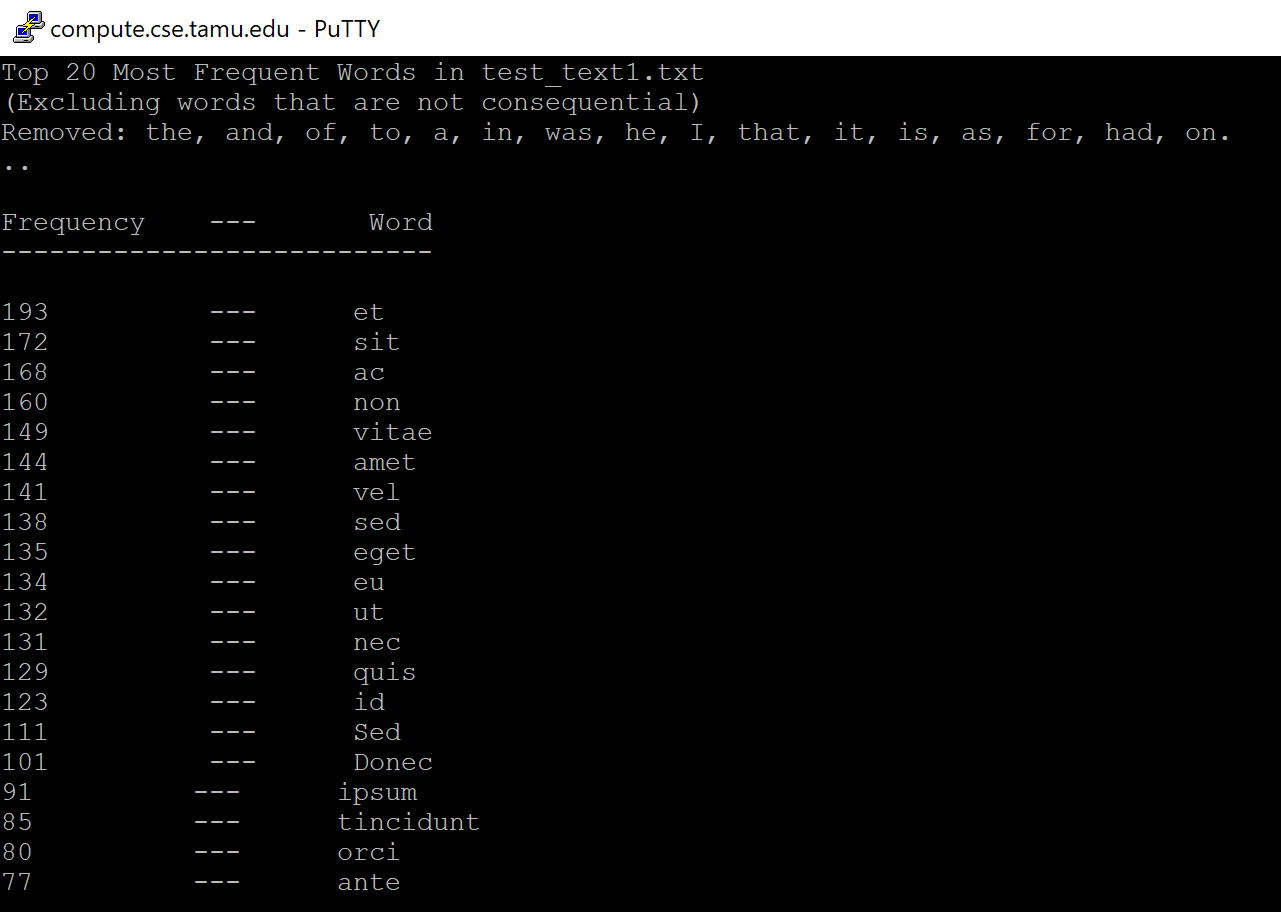
\includegraphics[width = 8 cm]{PUTTYBuildServerOutput-2.png}\ \\
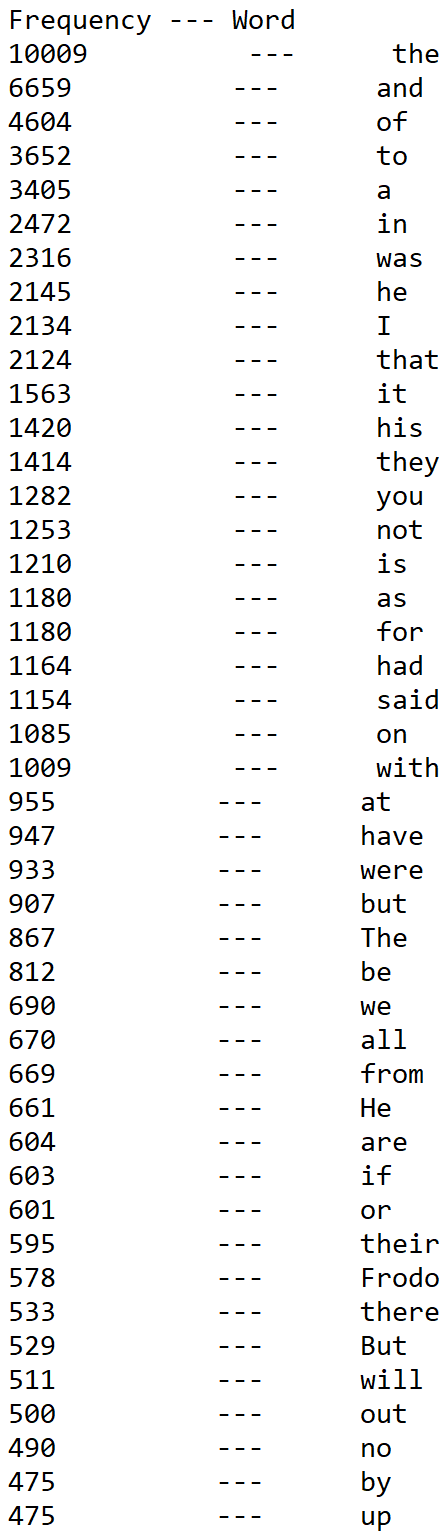
\includegraphics[height = 15 cm]{ListOfMostUsedWords.png}\ \\
\end{enumerate}
\end{itemize}

\section*{}
\begin{lyxcode}
\end{lyxcode}

\end{document}
